\documentclass{article}
\usepackage{amsmath,amssymb}
\usepackage{hyperref}
\usepackage{graphicx}
\usepackage{todonotes}

\title{\bf{Laboratory Project Three: Laser Doppler Velocimetry}}
\author{Nicholas Malaya \\ Department of Mechanical Engineering \\
University of Texas at Austin} \date{} 

\begin{document}
\maketitle
\date{}
\newpage
\section{Objectives}

\textbf{A short paragraph listing the specific objectives of this laboratory.}   

I believe the purpose of this laboratory was to learn about
several of the considerations necessary to properly operate an
LDV. Unlike the previous labs, the LDV had quite a bit of operational
details required to even begin gathering data. Our group took over an
hour to first start up the laser, play around with the oscilloscope,
etc. 

Beyond a familiarity with the LDV apparatus, this is also the first lab
where we have attempted to gather spatially resolved measurements. In
particular, we have characterized the free-stream turbulence (which we
expect to be statistically spatially independent) as well as the flow in
the wake of a cylinder. 

Common with the previous efforts, this work was also focused on
estimating the uncertainties (and ultimately, plausibility ) of our
measurements, both through uncertainty estimates as well as comparing
with available results in the literature. 

It was also my favorite lab. Felt very high tech. 

\section{Background and Experimental Details}

\textbf{Describe the basic operation of an LDV.}

I see the LDV as a four step process. 

\begin{itemize}
 \item Laser Crossing
 \item Particle movement through the fringes
 \item Light collected
 \item Signal postprocessing
\end{itemize}

Two laser beams cross, creating an interference pattern. Particles,
moving through this pattern reflect light in a similar oscillating
pattern, (some of) which is reflected back and collected. After signal
processing, the frequency of the signal of reflected light can be used
to calculate the quantity of interest, the particle's velocity. 

\textbf{Explain what frequency
shifting is, and why it is used.} 

We use frequency shifting so that we can measure flow
reversals. The frequency of light cannot be negative. 
If we did not shift the frequency of light scattered off
particles, we would have instances where particles moving backward
appeared to have the same frequency as particles moving
forward. Instead, by shifting the frequency forward, we can measure
frequencies that are lower than the effective frequency shift, which
permits us to determine the sign of the velocity.

\textbf{Calculate the size of the Probe Volume}

The size of the probe volume is given by Stavros on page 267, 
\begin{equation}
 V_p = \frac{\pi d_{fe}^3}{6\text{ Cos}(\theta/2)\text{
  Sin}(\theta/2)}. 
\end{equation}

$d_{fe}$ is the focused beam diameter, which is expressed on the same
page as,  
\begin{equation}
 d_{fe} \approx \frac{4f_T \lambda}{\pi d_e}
\end{equation}
with $f_T$ the lens focal length, $\lambda$ the laser wavelength, $d_e$
the beam diameter. The laser beam diameter was given as 1.3mm. The
wavelength of channel one was 514.5 nm, and channel two was 488 nm. The
lens focal length is 363mm for both beams. This provides an estimated
beam diameter of 0.1829 mm and 0.1735 mm. 

However, we also need $\theta/2$, the half intersection angle, here. We
can calculate this using, 
\begin{equation}
 \theta/2 = \text{tan}^{-1}\left(\frac{d/2}{f_T}\right)
\end{equation}
where d is the distance between beams and f is the focal length. For
both our beams, the focal length is 363 mm and the beam separation is 50
mm. This gives 0.687 radians or 3.94 degrees for the half angle. That
sounds approximately correct, the angle certainly appeared to be quite
shallow. 

Our probe volume then is expected to be, $0.001397 m^3$ for probe volume
one, and $0.001325 m^3$ for probe volume two. 

 \textbf{Calculate the expected frequency response of the glass sphere seed particles.}

Stavros give the characteristic time of the particles as, 
\begin{equation}
 \tau_p = \frac{\rho_P d_p^2}{18 \mu_F}
\end{equation}
where $\rho_p $ and $d_p$ are the density and diameters of the
particles, respectively. $\mu_F$ is the dynamic viscosity of the fluid. 
This provides a characteristic frequency, as
\begin{equation}
 \omega_c = 1/\tau_p.
\end{equation}
This is important because this represents the highest frequency of
turbulent fluctuation that the particles could accurately track in a
flow. With diameters of 12 $\mu m$ (this will give the most restrictive
frequency) and density of $1.1$ g/cc, we find a frequency response of 47
KHz. 

This now naturally bears questioning: are we actually able to resolve the
velocities we are measuring? The doppler frequency is measured as,
\begin{equation}
 f_d = u_x / d_f 
\end{equation}
Where $u_x = 0.42 m/s$ and $d_f$ is given as $3.75 \mu m$. Our doppler
frequency is therefore 112 kHz, which is higher than our mean. However,
the mean does not change, so the particles naturally equilibrate. A more
meaningful measure is the RMS, which is on the order of the velocity
fluctuations. This is in general much smaller than 0.42, and in the
freestream, was $\approx 0.01$, giving a doppler frequency of just 2
kHz. We can easily measure this. We expect to be able to resolve roughly
any fluctuations less than 0.2 m/s, which is more than
any fluctuations observed in our runs. 

% the doppler frequency of the particle is the normal velocity over the
% fringe spacing, which was: X-direction: 3.744um; y-direction: 3.551um
% (taken from Flowsizer) 


\section{Experiment One: Freestream}

\textbf{Indicate the frequency shift and bandpass filter settings used,
and why.} 

The Bragg cell shifts by 40 MHz. Our downmix frequency was set to 39.85
for channel one, and 39.95 for channel two. The different settings were
due to the fact that the velocity components have different mean
velocities ($\approx 0.41$ and 0) and so produce a different shift. As a
result of this downmix, our effective shifting frequency was 150kHz (and
50 kHz for channel 2). As mentioned in the previous section, the mean
velocity shifts the doppler from the particles by as much as 112 kHz,
meaning that for both our cases, our total 
frequency response was about 40-50kHz, which fits right in our
bandpass region of 10-100kHz.   

We visually verified that the histograms were well centered in our
bandpass region, and that the tails were not being cut off. 

% add histogram showing it is not cut off?
   % \begin{figure}[!htb]
   %  \begin{center}
   %   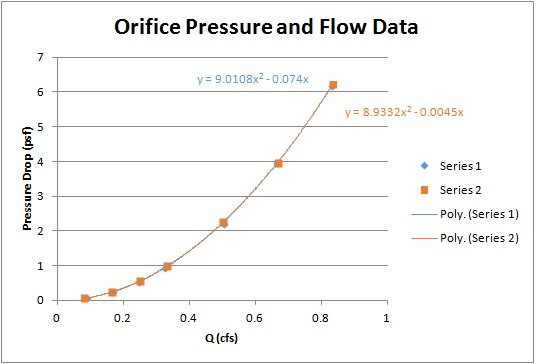
\includegraphics[width = 12 cm]{figs/Q_dP_fits.jpg}
   %   \caption{}
   %   \label{orif-zoom}
   %  \end{center}
   % \end{figure}

\textbf{Indicate the laser power and PMT voltage settings used, and why
these values were selected.} 

The PMT for channel one was 600 V, and 500 for channel two. The laser
power was set at 1 W. We did not adjust the laser power much at all, as
we started with a reasonable count number. We did adjust the PMT down
for channel two because the number of events was much higher than the
freestream, and we were trying to get slightly more even numbers of
counts. 

\textbf{Indicate the ``Burst Threshold'' and ``SNR'' settings used, and why
these values were selected.} 


The burst threshold was set to 30 mV and 60 mV for channel's one and
two, respectively. We used a higher burst threshold for channel two
because the mean was typically zero here, and we were getting lower data
rates.\todo{do you believe this?} 

We set the SNR settings to ``very low'' because our burst efficiencies
were always quite high (often above 80\%). The lab guidelines mentioned
that anything over 50\% is good, so we felt there was no need to further
filter the data beyond the minimum settings. 

We would often look at the oscilloscope to examine the bursts incoming. 
After adjustment, we had very smooth and continuous (with reasonable
amplitude) bursts appearing. We thought that this was an indication that
the laser and signal processing was working quite well. Our filters were
much higher than the ambient noise, but seldom higher than obviously
incoming signals, so we were also happy with the settings in that
context. 

These settings were used both both the freestream as well as the wake
measurements, so that we could make direct comparisons between data
gathered at each point. 

%
% add chart of oscilloscope?
%
%

\textbf{Present the mean and RMS velocities measured, including
uncertainties for these measurements.} 

The mean and RMS for the freestream velocity were measured as, 
-0.4141 m/s and 0.00328 m/s, respectively. These were calculated by
taking the mean of 5 samples from the LDV. However, each of these
samples was taken from 2000 samples aggregated together as a
histogram. Thus, the uncertainty of these calculations
can be gleaned from our estimate of the of the variance of the mean, or
the ``sample error'', $2\sigma/\sqrt{n}$. This provides uncertainty
estimates of, .0016 m/s for the mean, e.g. $0.4141 \pm
0.0016$ which is 0.3\%. Likewise, our estimate for the uncertainty in the
streamwise RMS is 0.0002072 m/s, giving, $0.00328 m/s \pm 0.0002072$ or
about 6\%. We estimate the average and precision uncertainty for the v
mean and RMS as, $0.00344 m/s \pm 4.8e-5$ (1.4\%) and $0.00168 m/s \pm
6.7e-4$ (3.9\%). 

These numbers seem reasonable to me. The fluctuating turbulence
provides an inherent variability, but we were throwing a fair number of
samples at the problem (2000) and this was resulting in very smooth
histograms. Furthermore, unlike the next results section, these
histrograms were not particularly skewed, but were evenly distributed
around the mean. The PDFs were not quite gaussian, with some visible
kurtosis, so they did exhibit some tendencies towards extreme events,
which we likely did have trouble catching with our sample
size.\todo{bias estimate}



\textbf{Comment on the turbulence intensities,
$\frac{u_{\text{rms}}}{U}$ and $\frac{v_{\text{rms}}}{U}$, do they make sense?}

$\frac{v_{\text{rms}}}{U}$ certainly does not as measured on the
laboratory equipment. I suspect that this was actually
$\frac{v_{\text{rms}}}{V}$, which was dividing essentially by a small number,
because the turbulence intensities were often shown to exceed 40\%. 
$\frac{u_{\text{rms}}}{U}$ (the freestream component) appeared to be
reasonable. We observed turbulence intensities slightly below one
percent. 

Calculating the turbulence intensities from our raw data, we found that
the freestream intensity was $0.00793 \pm 0.000510$, or less than one
percent in magnitude, and slightly less than six (relative to the
average ) percent uncertainty on that number. Likewise, the spanwise
velocity measurements were $0.004065 \pm 0.00015$ and an uncertainty of
closer to 4\%. I'll admit this result surprised me.
I expect the flow is roughly isotropic, since we are not near any walls. 
Thus, I expected the turbulence intensities to be about the same as
well. However, they are patently not, and they are farther apart than
our uncertainty bounds, so I expect this is a real effect. Otherwise,
the turbulence intensity levels are roughly about where we would expect
them to be for free-stream turbulence. 

% As for the bias stuff, I'm just looking at the equation he gave us in
% Lecture 13 where U_meas/U_actual=1+(u_rms/U)^2.  Calculating the right
% half gives values of ~1.03 for the higher turbulence intensities and
% ~1-1.01 for the lower, which seems to match up with the ranges he told
% us. 

\section{Experiment Two: Wake Measurements}

\textbf{Present results from your wake measurements, including
uncertainty of the measurements. Compare your results with data in the
literature and comment on similarities and differences. } 

I am comparing the wake measurements to an interesting paper by Ong and
Wallace, entitled, ``The velocity field of the turbulent very near wake
of a circular cylinder''. I like this paper because it provides
measurements from circular cylinders at Reynolds numbers approximately
near our conditions (Re $\approx 2000$ versus 3900, versus many papers
at substantially larger Re) and at values that are nominally identical
to our location, e.g. $x/d < 10$. A deficiency of this paper for our
purposes is that the measurements were conducted with a hot wire, and
not the present LDV system. 

We measured the diameter of the cylinder with a set of calipers. 
for a $d=0.374$ inches we desire to measure 5d downstream, or $1.87$
inches. We then moved another 1.87 inches and repeated out measurements
(10d). However, we had to convert from inches to mm for the arm
readings. This I wrote down as, $d=0.374$ inches or $9.5$ mm, so $5d =
47.5 mm$. The arm moves 1/10mm, so 475 was the reading placed into the
box to move the laser. We then checked both times the distance with the
micrometer, and it appeared to be correct. 

In order to investigate the histeresis and repeatability of our
measurements, we started at zero, moved down two diameter widths, then
back up through to positive two diameters, and then back down to
zero. We ``snaked'' through. In this way, we made a clean sweep through
two full sets of data, while simultaneously approaching from a different
direction for each set. 

\begin{figure}[!htb]
 \begin{center}
  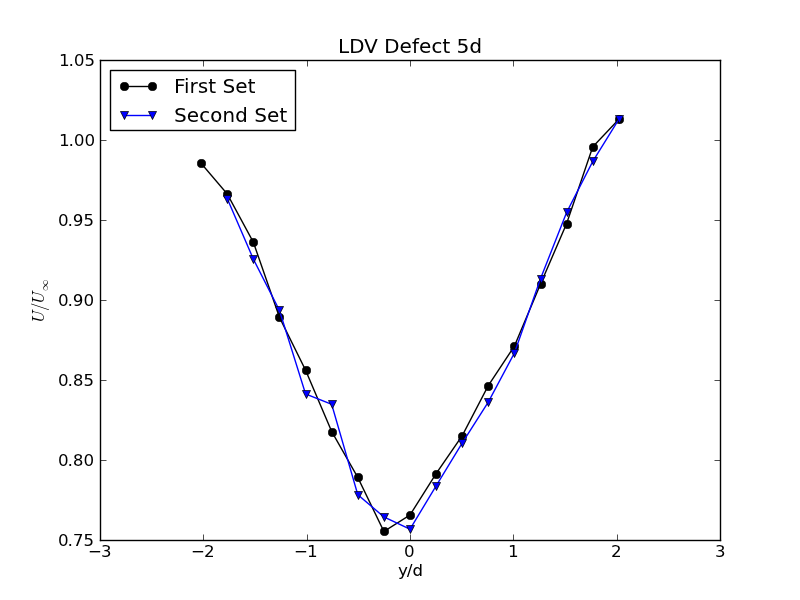
\includegraphics[width = 12 cm]{figs/defect}
  \caption{The streamwise velocity normalize by freestream velocity. We
  show both sets for a discussion of repeatability.}
  \label{repeat}
 \end{center}
\end{figure}

The streamwise velocity is shown in figure \ref{repeat}. Both repeated
experiments are shown. The good news is that the data is relatively
repeatable, with each point somewhat close to the other set. 
Immediately one sees a major issue with the data,
namely, that several anomalous data points exist. For instance, in the
first data set, the point slightly less than zero at $y/d=0.25$ is
actually lower than the point directly behind the cylinder. Was this
just a very bad data point, or did some other more systematic error
appear? It is not clear, but it gives the appearance of skewness to the
entire output. Another issue is that we clearly did not take enough
points past $y/d=2$. From our literature search we had believed that
this was far enough to go to be back into the freestream, and actually
the data appears to support this, but we should have taken more points
so as to ensure that this is indeed truly the case, and that the points
beyond $y/d=2$ do continue to flatten out.

So far, this data compares reasonably well with the literature. The
bottom of our peak (at the centerline) corresponds to a value of
0.75. The paper by Ong et al. has a minimum at 5d of 0.73, which is at
least close, if not completely identical. Some of this difference might
be attributable the different reynolds numbers between the cases. 

\begin{figure}[!htb]
 \begin{center}
  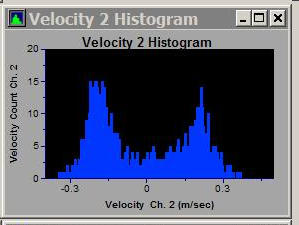
\includegraphics[width = 12 cm]{figs/backflow}
  \caption{The spanwise velocity at the centerline is
  significantly bimodal. }
  \label{back}
 \end{center}
\end{figure}

Notice that near the centerline we found significantly bimodal
distributions of velocity in the spanwise component of velocity. This is
shown in figure \ref{back}. This is as expected, because the spanwise
velocity is either going above or below the cylinder, and that tends to
favorably impart a spanwise velocity as it does. While at the centerline
these components were competing, above and below the centerline this
introduced considerable skewness in the observed histograms of spanwise
velocity. 

\begin{figure}[!htb]
 \begin{center}
  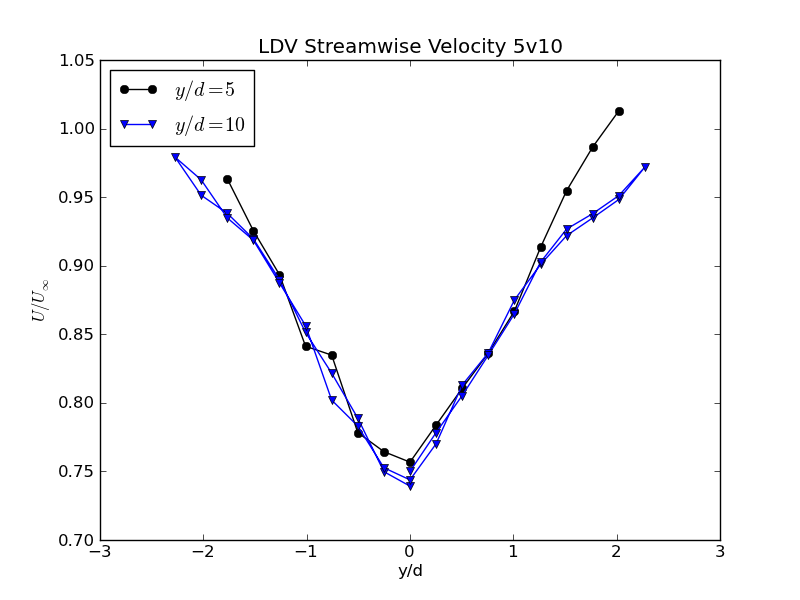
\includegraphics[width = 12 cm]{figs/defect10}
  \caption{A comparison between the five and ten cylinder diameters
  streamwise velocity profiles.}
  \label{back}
 \end{center}
\end{figure}

An comparison between the mean velocity for 5 and 10 cylinder diameters
is shown in figure \ref{back}. It is very difficult to tell if this
is in agreement with the literature. What appears clear is that the data
for the streamwise velocities are close to each other even at a spacing
of 5 diameters. Our data appears consistent with the literature, in that
the wake region is broader at ten diameters. I looked at Pope to try to
quantitatively estimate how much it should grow, as if it was a
freestream jet, and the radius is the jet half-width. However, I
couldn't munge this into anything particularly interesting. In short,
while the fact these profiles are roughly equivalent surprised me, I
cannot find any evidence they should be exhibiting greater differences. 

\begin{figure}[!htb]
 \begin{center}
  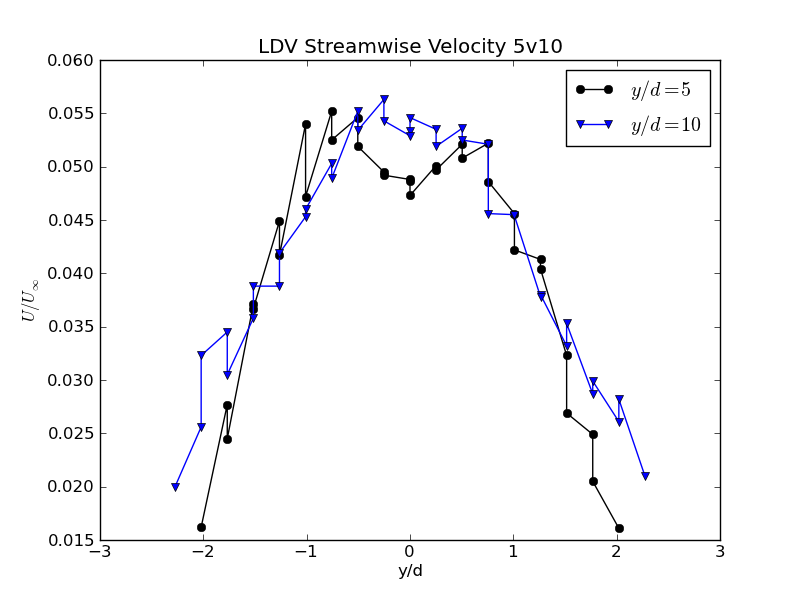
\includegraphics[width = 12 cm]{figs/urms}
  \caption{The five and ten diameter distances $U_{rms}$ profiles. }
  \label{urms}
 \end{center}
\end{figure}

In figure \ref{urms} we plot the five and ten diameter $U_{rms}$
profiles. First, the good news: the magnitudes of our measurements were
largely consistent with the values in the literature, with a sharp peak
existing below 0.6. Our five diameter measurements show, very modestly,
the characteristic double peak off center of the cylinder, which is also
consistent with our expectations. However, our data is noisy and did not
well resolve the peaks. We also did not take enough points around $|y/d|
=1$ to really resolve this peak. Furthermore, our colleagues paper
clearly shows a similar (although smaller) double peak at the
centerline, which we appear to have not captured at all. At this point I
am concerned that we did not measure the $y/d$ distance correctly, but
we really were very careful and did have an independent check (Nick did
it and it was checked by Owen). 

The uncertainty was bounded in estimation using either the repeated
measurements at the center ($y=0$) where the turbulence was at a peak,
versus the freestream uncertainty estimates provided previously. We
expect that the freestream is more accurate away from the cylinder, but
an underestimate of the variability as you approach the centerline. Vice
versa, the centerline error would be more accurate near the center, but
overestimating the uncertainty near the freestream. \todo{finish me!}

\section{Conclusions}

\textbf{Conclude by giving your opinion about whether your measurements
are more or less reliable than measurements in the literature.} 

I absolutely do not believe our measurements are more accurate than the
rival paper. I'll admit I am somewhat disappointed in the results
presented here, but in particular given the shortcomings presented in
the previous section with respect to several anomalous points, I would
want to perform additional measurements. 

In theory, however, I do believe that an LDV could be accurate. Some of
the major disadvantages of LDV are the cost and the problems associated
with near wall features. However, neither of those impact the
measurements here. While we needed to perform more measurements and
possibly more laser and sensor adjustments, the LDV I believe in
principle can be more accurate than it appears here. Another
advantage of the LDV is that it can measure backflow which as mentioned
previously appeared in the spanwise component of velocity. 



%
%
%
\end{document}

% LocalWords:  reynolds H20 piecewise RDG yar
